% Options for packages loaded elsewhere
\PassOptionsToPackage{unicode}{hyperref}
\PassOptionsToPackage{hyphens}{url}
%
\documentclass[
]{article}
\usepackage{amsmath,amssymb}
\usepackage{iftex}
\ifPDFTeX
  \usepackage[T1]{fontenc}
  \usepackage[utf8]{inputenc}
  \usepackage{textcomp} % provide euro and other symbols
\else % if luatex or xetex
  \usepackage{unicode-math} % this also loads fontspec
  \defaultfontfeatures{Scale=MatchLowercase}
  \defaultfontfeatures[\rmfamily]{Ligatures=TeX,Scale=1}
\fi
\usepackage{lmodern}
\ifPDFTeX\else
  % xetex/luatex font selection
\fi
% Use upquote if available, for straight quotes in verbatim environments
\IfFileExists{upquote.sty}{\usepackage{upquote}}{}
\IfFileExists{microtype.sty}{% use microtype if available
  \usepackage[]{microtype}
  \UseMicrotypeSet[protrusion]{basicmath} % disable protrusion for tt fonts
}{}
\makeatletter
\@ifundefined{KOMAClassName}{% if non-KOMA class
  \IfFileExists{parskip.sty}{%
    \usepackage{parskip}
  }{% else
    \setlength{\parindent}{0pt}
    \setlength{\parskip}{6pt plus 2pt minus 1pt}}
}{% if KOMA class
  \KOMAoptions{parskip=half}}
\makeatother
\usepackage{xcolor}
\usepackage[margin=1in]{geometry}
\usepackage{color}
\usepackage{fancyvrb}
\newcommand{\VerbBar}{|}
\newcommand{\VERB}{\Verb[commandchars=\\\{\}]}
\DefineVerbatimEnvironment{Highlighting}{Verbatim}{commandchars=\\\{\}}
% Add ',fontsize=\small' for more characters per line
\usepackage{framed}
\definecolor{shadecolor}{RGB}{248,248,248}
\newenvironment{Shaded}{\begin{snugshade}}{\end{snugshade}}
\newcommand{\AlertTok}[1]{\textcolor[rgb]{0.94,0.16,0.16}{#1}}
\newcommand{\AnnotationTok}[1]{\textcolor[rgb]{0.56,0.35,0.01}{\textbf{\textit{#1}}}}
\newcommand{\AttributeTok}[1]{\textcolor[rgb]{0.13,0.29,0.53}{#1}}
\newcommand{\BaseNTok}[1]{\textcolor[rgb]{0.00,0.00,0.81}{#1}}
\newcommand{\BuiltInTok}[1]{#1}
\newcommand{\CharTok}[1]{\textcolor[rgb]{0.31,0.60,0.02}{#1}}
\newcommand{\CommentTok}[1]{\textcolor[rgb]{0.56,0.35,0.01}{\textit{#1}}}
\newcommand{\CommentVarTok}[1]{\textcolor[rgb]{0.56,0.35,0.01}{\textbf{\textit{#1}}}}
\newcommand{\ConstantTok}[1]{\textcolor[rgb]{0.56,0.35,0.01}{#1}}
\newcommand{\ControlFlowTok}[1]{\textcolor[rgb]{0.13,0.29,0.53}{\textbf{#1}}}
\newcommand{\DataTypeTok}[1]{\textcolor[rgb]{0.13,0.29,0.53}{#1}}
\newcommand{\DecValTok}[1]{\textcolor[rgb]{0.00,0.00,0.81}{#1}}
\newcommand{\DocumentationTok}[1]{\textcolor[rgb]{0.56,0.35,0.01}{\textbf{\textit{#1}}}}
\newcommand{\ErrorTok}[1]{\textcolor[rgb]{0.64,0.00,0.00}{\textbf{#1}}}
\newcommand{\ExtensionTok}[1]{#1}
\newcommand{\FloatTok}[1]{\textcolor[rgb]{0.00,0.00,0.81}{#1}}
\newcommand{\FunctionTok}[1]{\textcolor[rgb]{0.13,0.29,0.53}{\textbf{#1}}}
\newcommand{\ImportTok}[1]{#1}
\newcommand{\InformationTok}[1]{\textcolor[rgb]{0.56,0.35,0.01}{\textbf{\textit{#1}}}}
\newcommand{\KeywordTok}[1]{\textcolor[rgb]{0.13,0.29,0.53}{\textbf{#1}}}
\newcommand{\NormalTok}[1]{#1}
\newcommand{\OperatorTok}[1]{\textcolor[rgb]{0.81,0.36,0.00}{\textbf{#1}}}
\newcommand{\OtherTok}[1]{\textcolor[rgb]{0.56,0.35,0.01}{#1}}
\newcommand{\PreprocessorTok}[1]{\textcolor[rgb]{0.56,0.35,0.01}{\textit{#1}}}
\newcommand{\RegionMarkerTok}[1]{#1}
\newcommand{\SpecialCharTok}[1]{\textcolor[rgb]{0.81,0.36,0.00}{\textbf{#1}}}
\newcommand{\SpecialStringTok}[1]{\textcolor[rgb]{0.31,0.60,0.02}{#1}}
\newcommand{\StringTok}[1]{\textcolor[rgb]{0.31,0.60,0.02}{#1}}
\newcommand{\VariableTok}[1]{\textcolor[rgb]{0.00,0.00,0.00}{#1}}
\newcommand{\VerbatimStringTok}[1]{\textcolor[rgb]{0.31,0.60,0.02}{#1}}
\newcommand{\WarningTok}[1]{\textcolor[rgb]{0.56,0.35,0.01}{\textbf{\textit{#1}}}}
\usepackage{longtable,booktabs,array}
\usepackage{calc} % for calculating minipage widths
% Correct order of tables after \paragraph or \subparagraph
\usepackage{etoolbox}
\makeatletter
\patchcmd\longtable{\par}{\if@noskipsec\mbox{}\fi\par}{}{}
\makeatother
% Allow footnotes in longtable head/foot
\IfFileExists{footnotehyper.sty}{\usepackage{footnotehyper}}{\usepackage{footnote}}
\makesavenoteenv{longtable}
\usepackage{graphicx}
\makeatletter
\def\maxwidth{\ifdim\Gin@nat@width>\linewidth\linewidth\else\Gin@nat@width\fi}
\def\maxheight{\ifdim\Gin@nat@height>\textheight\textheight\else\Gin@nat@height\fi}
\makeatother
% Scale images if necessary, so that they will not overflow the page
% margins by default, and it is still possible to overwrite the defaults
% using explicit options in \includegraphics[width, height, ...]{}
\setkeys{Gin}{width=\maxwidth,height=\maxheight,keepaspectratio}
% Set default figure placement to htbp
\makeatletter
\def\fps@figure{htbp}
\makeatother
\setlength{\emergencystretch}{3em} % prevent overfull lines
\providecommand{\tightlist}{%
  \setlength{\itemsep}{0pt}\setlength{\parskip}{0pt}}
\setcounter{secnumdepth}{-\maxdimen} % remove section numbering
% definitions for citeproc citations
\NewDocumentCommand\citeproctext{}{}
\NewDocumentCommand\citeproc{mm}{%
  \begingroup\def\citeproctext{#2}\cite{#1}\endgroup}
\makeatletter
 % allow citations to break across lines
 \let\@cite@ofmt\@firstofone
 % avoid brackets around text for \cite:
 \def\@biblabel#1{}
 \def\@cite#1#2{{#1\if@tempswa , #2\fi}}
\makeatother
\newlength{\cslhangindent}
\setlength{\cslhangindent}{1.5em}
\newlength{\csllabelwidth}
\setlength{\csllabelwidth}{3em}
\newenvironment{CSLReferences}[2] % #1 hanging-indent, #2 entry-spacing
 {\begin{list}{}{%
  \setlength{\itemindent}{0pt}
  \setlength{\leftmargin}{0pt}
  \setlength{\parsep}{0pt}
  % turn on hanging indent if param 1 is 1
  \ifodd #1
   \setlength{\leftmargin}{\cslhangindent}
   \setlength{\itemindent}{-1\cslhangindent}
  \fi
  % set entry spacing
  \setlength{\itemsep}{#2\baselineskip}}}
 {\end{list}}
\usepackage{calc}
\newcommand{\CSLBlock}[1]{\hfill\break\parbox[t]{\linewidth}{\strut\ignorespaces#1\strut}}
\newcommand{\CSLLeftMargin}[1]{\parbox[t]{\csllabelwidth}{\strut#1\strut}}
\newcommand{\CSLRightInline}[1]{\parbox[t]{\linewidth - \csllabelwidth}{\strut#1\strut}}
\newcommand{\CSLIndent}[1]{\hspace{\cslhangindent}#1}
\ifLuaTeX
  \usepackage{selnolig}  % disable illegal ligatures
\fi
\usepackage{bookmark}
\IfFileExists{xurl.sty}{\usepackage{xurl}}{} % add URL line breaks if available
\urlstyle{same}
\hypersetup{
  pdftitle={index},
  hidelinks,
  pdfcreator={LaTeX via pandoc}}

\title{index}
\author{}
\date{\vspace{-2.5em}2024-09-21}

\begin{document}
\maketitle

\subsection{Sinistros de trânsito na base do
SIM-SUS}\label{sinistros-de-truxe2nsito-na-base-do-sim-sus}

O código a seguir lerá todos os anos da base do SIM-SUS como um único
dataframe. Como o interesse neste documento é a quantidade de mortes no
trânsito, serão selecionadas somente as colunas de DTOBITO e CAUSABAS.
De modo a calcular os números por ano, uma coluna de ano será criada a
partir de DTOBITO.

\begin{Shaded}
\begin{Highlighting}[]
\CommentTok{\# Importar bibliotecas necessárias}
\FunctionTok{library}\NormalTok{(}\StringTok{\textquotesingle{}read.dbc\textquotesingle{}}\NormalTok{)}

\CommentTok{\# Ler arquivos originais compactados em .dbc como dataframes}
\NormalTok{sim\_sus }\OtherTok{\textless{}{-}} \FunctionTok{list.files}\NormalTok{(}\AttributeTok{path       =}\NormalTok{ sim\_sus\_folder, }
                      \AttributeTok{pattern    =} \StringTok{\textquotesingle{}DOEXT...DBC\textquotesingle{}}\NormalTok{,}
                      \AttributeTok{recursive  =} \ConstantTok{FALSE}\NormalTok{,}
                      \AttributeTok{full.names =} \ConstantTok{TRUE}\NormalTok{)}

\NormalTok{sim\_sus }\OtherTok{\textless{}{-}}\NormalTok{ sim\_sus }\SpecialCharTok{\%\textgreater{}\%} \FunctionTok{map\_df}\NormalTok{(read.dbc) }\SpecialCharTok{\%\textgreater{}\%} \FunctionTok{as\_tibble}\NormalTok{()}

\CommentTok{\# Selecionar colunas de interesse para ocorrências de trânsito}
\NormalTok{sim\_sus }\OtherTok{\textless{}{-}}\NormalTok{ sim\_sus }\SpecialCharTok{\%\textgreater{}\%} \FunctionTok{select}\NormalTok{(DTOBITO, CAUSABAS)}

\CommentTok{\# Criar coluna de ano da morte}
\NormalTok{sim\_sus }\OtherTok{\textless{}{-}}\NormalTok{ sim\_sus }\SpecialCharTok{\%\textgreater{}\%} \FunctionTok{mutate}\NormalTok{(}\AttributeTok{ANOOBITO =} \FunctionTok{str\_sub}\NormalTok{(.}\SpecialCharTok{$}\NormalTok{DTOBITO, }\SpecialCharTok{{-}}\DecValTok{4}\NormalTok{), }\AttributeTok{.before =} \StringTok{\textquotesingle{}DTOBITO\textquotesingle{}}\NormalTok{)}
\end{Highlighting}
\end{Shaded}

As causas básicas da CID-10 a serem consideradas como sinistros de
trânsito são definidas no documento \textbf{WHO methods and data sources
for country-level causes of death 2000-2019} {[}Métodos e fontes de
dados da OMS para as causas de morte a nível nacional 2000-2019{]}
(\citeproc{ref-who2020}{WHO, 2020}). Para países em que a CID-10 possui
quatro caracteres, como é o caso do Brasil, os códigos a serem filtrados
são os seguintes:

\begin{verbatim}
ICD-10 codes: V01-V04, V06 (.1-.9), V09 (.2-.3), V10- V14 (.3-.9), V15-V19 (.4-.9), V20-V28 (.3-.9), V29- V79 (.4-.9), V80 (.3-.5), V81.1, V82 (.1, .8-.9), V83-V86 (.0-.3), V87 (.0-.9), V89 (.2-.3, .9), V99, Y85.0
\end{verbatim}

O código em R para executar este filtro é apresentado a seguir.

\begin{Shaded}
\begin{Highlighting}[]
\CommentTok{\# Road injuries}
\NormalTok{road\_injuries }\OtherTok{\textless{}{-}}
\NormalTok{  sim\_sus }\SpecialCharTok{\%\textgreater{}\%}
  \FunctionTok{filter}\NormalTok{(}
    \FunctionTok{str\_starts}\NormalTok{(CAUSABAS, }\StringTok{\textquotesingle{}V0[12346][1{-}9]\textquotesingle{}}\NormalTok{) }\SpecialCharTok{|} \FunctionTok{str\_starts}\NormalTok{(CAUSABAS, }\StringTok{\textquotesingle{}V09[2{-}3]\textquotesingle{}}\NormalTok{) }\SpecialCharTok{|}
    \FunctionTok{str\_starts}\NormalTok{(CAUSABAS, }\StringTok{\textquotesingle{}V1[0{-}4][3{-}9]\textquotesingle{}}\NormalTok{) }\SpecialCharTok{|} \FunctionTok{str\_starts}\NormalTok{(CAUSABAS, }\StringTok{\textquotesingle{}V1[5{-}9][4{-}9]\textquotesingle{}}\NormalTok{) }\SpecialCharTok{|}
    \FunctionTok{str\_starts}\NormalTok{(CAUSABAS, }\StringTok{\textquotesingle{}V2[0{-}8][3{-}9]\textquotesingle{}}\NormalTok{) }\SpecialCharTok{|} \FunctionTok{str\_starts}\NormalTok{(CAUSABAS, }\StringTok{\textquotesingle{}V29[4{-}9]\textquotesingle{}}\NormalTok{) }\SpecialCharTok{|}
    \FunctionTok{str\_starts}\NormalTok{(CAUSABAS, }\StringTok{\textquotesingle{}V[3{-}7][0{-}9][4{-}9]\textquotesingle{}}\NormalTok{) }\SpecialCharTok{|}
    \FunctionTok{str\_starts}\NormalTok{(CAUSABAS, }\StringTok{\textquotesingle{}V80[3{-}5]\textquotesingle{}}\NormalTok{) }\SpecialCharTok{|} \FunctionTok{str\_starts}\NormalTok{(CAUSABAS, }\StringTok{\textquotesingle{}V8[12]1\textquotesingle{}}\NormalTok{) }\SpecialCharTok{|}
    \FunctionTok{str\_starts}\NormalTok{(CAUSABAS, }\StringTok{\textquotesingle{}V82[8{-}9]\textquotesingle{}}\NormalTok{) }\SpecialCharTok{|} \FunctionTok{str\_starts}\NormalTok{(CAUSABAS, }\StringTok{\textquotesingle{}V8[3{-}6][0{-}3]\textquotesingle{}}\NormalTok{) }\SpecialCharTok{|}
    \FunctionTok{str\_starts}\NormalTok{(CAUSABAS, }\StringTok{\textquotesingle{}V87[0{-}9]\textquotesingle{}}\NormalTok{) }\SpecialCharTok{|} \FunctionTok{str\_starts}\NormalTok{(CAUSABAS, }\StringTok{\textquotesingle{}V89[239]\textquotesingle{}}\NormalTok{) }\SpecialCharTok{|}
    \FunctionTok{str\_starts}\NormalTok{(CAUSABAS, }\StringTok{\textquotesingle{}V99\textquotesingle{}}\NormalTok{) }\SpecialCharTok{|} \FunctionTok{str\_starts}\NormalTok{(CAUSABAS, }\StringTok{\textquotesingle{}Y85\textquotesingle{}}\NormalTok{)}
\NormalTok{  ) }\SpecialCharTok{\%\textgreater{}\%}
  \FunctionTok{group\_by}\NormalTok{(ANOOBITO) }\SpecialCharTok{\%\textgreater{}\%}
  \FunctionTok{tally}\NormalTok{() }\SpecialCharTok{\%\textgreater{}\%}
  \FunctionTok{ungroup}\NormalTok{() }\SpecialCharTok{\%\textgreater{}\%}
  \FunctionTok{rename}\NormalTok{(}\AttributeTok{road\_injuries =}\NormalTok{ n)}
\end{Highlighting}
\end{Shaded}

\begin{Shaded}
\begin{Highlighting}[]
\NormalTok{road\_injuries}
\end{Highlighting}
\end{Shaded}

\begin{longtable}[]{@{}cc@{}}
\toprule\noalign{}
Ano de óbito & Total \\
\midrule\noalign{}
\endhead
\bottomrule\noalign{}
\endlastfoot
2011 & 41.775 \\
2012 & 43.184 \\
2013 & 40.858 \\
2014 & 42.256 \\
2015 & 37.346 \\
2016 & 36.196 \\
2017 & 34.346 \\
2018 & 31.580 \\
2019 & 30.883 \\
2020 & 31.669 \\
2021 & 33.010 \\
2022 & 33.030 \\
2023 & 32.922 \\
\end{longtable}

Utilizados desta forma, resultarão nos mesmos números apresentados na
plataforma \textbf{WHO Mortality Database - Road Traffic Accidents}
{[}Base de Mortalidade da OMS - Sinistros de Trânsito{]}
(\citeproc{ref-who2022}{WHO, 2022}), que possui dados para o Brasil até
o ano de 2020.

\subsection{Baixando as bases do SIM-SUS pelo
R}\label{baixando-as-bases-do-sim-sus-pelo-r}

No R, o seguinte código vai baixar os arquivos para os anos de 2011 a
2023.

\begin{Shaded}
\begin{Highlighting}[]
\CommentTok{\# Importar bibliotecas necessárias}
\FunctionTok{library}\NormalTok{(}\StringTok{\textquotesingle{}tidyverse\textquotesingle{}}\NormalTok{)}
\FunctionTok{library}\NormalTok{(}\StringTok{\textquotesingle{}tidylog\textquotesingle{}}\NormalTok{)}
\FunctionTok{library}\NormalTok{(}\StringTok{\textquotesingle{}read.dbc\textquotesingle{}}\NormalTok{)}

\CommentTok{\# Pasta para armazenamento dos dados}
\NormalTok{sim\_sus\_folder }\OtherTok{\textless{}{-}} \FunctionTok{sprintf}\NormalTok{(}\StringTok{\textquotesingle{}\%s/dados\textquotesingle{}}\NormalTok{, }\FunctionTok{getwd}\NormalTok{())}
\FunctionTok{dir.create}\NormalTok{(sim\_sus\_folder, }\AttributeTok{recursive =} \ConstantTok{TRUE}\NormalTok{, }\AttributeTok{showWarnings =} \ConstantTok{FALSE}\NormalTok{)}

\CommentTok{\# Definir anos de início e de fim}
\NormalTok{ano\_inicial }\OtherTok{\textless{}{-}} \DecValTok{11}\NormalTok{; ano\_final }\OtherTok{\textless{}{-}} \DecValTok{23}
\NormalTok{base\_url }\OtherTok{\textless{}{-}} \StringTok{\textquotesingle{}ftp://ftp.datasus.gov.br/dissemin/publicos/SIM\textquotesingle{}}
\CommentTok{\# Puxar as bases de dados}
\ControlFlowTok{for}\NormalTok{ (ano }\ControlFlowTok{in} \FunctionTok{seq}\NormalTok{(ano\_inicial, ano\_final)) \{}
  \CommentTok{\# Baixar somente se arquivo ainda não existir na pasta}
\NormalTok{  dbc\_file }\OtherTok{\textless{}{-}} \FunctionTok{sprintf}\NormalTok{(}\StringTok{\textquotesingle{}\%s/DOEXT\%s.DBC\textquotesingle{}}\NormalTok{, sim\_sus\_folder, ano)}
  \ControlFlowTok{if}\NormalTok{ (}\SpecialCharTok{!}\FunctionTok{file.exists}\NormalTok{(dbc\_file)) \{}
\NormalTok{    url }\OtherTok{\textless{}{-}} \FunctionTok{sprintf}\NormalTok{(}\StringTok{\textquotesingle{}\%s/CID10/DOFET/DOEXT\%s.DBC\textquotesingle{}}\NormalTok{, base\_url, ano)}
\NormalTok{    result }\OtherTok{\textless{}{-}} \FunctionTok{try}\NormalTok{(\{ }\FunctionTok{download.file}\NormalTok{(url, dbc\_file)\} , }\AttributeTok{silent =} \ConstantTok{TRUE}\NormalTok{)}
    \CommentTok{\# Se arquivo consolidado não existir, tentar versão preliminar}
    \ControlFlowTok{if}\NormalTok{ (}\FunctionTok{class}\NormalTok{(result) }\SpecialCharTok{==} \StringTok{"try{-}error"}\NormalTok{) \{}
\NormalTok{      url }\OtherTok{\textless{}{-}} \FunctionTok{sprintf}\NormalTok{(}\StringTok{\textquotesingle{}/PRELIM/DOFET/DOEXT\%s.DBC\textquotesingle{}}\NormalTok{, base\_url, ano)}
      \FunctionTok{download.file}\NormalTok{(url, dbc\_file)}
\NormalTok{    \}}
\NormalTok{  \}}
\NormalTok{\}}
\end{Highlighting}
\end{Shaded}

\subsection{Como baixar as bases do SIM-SUS (modo
manual)}\label{como-baixar-as-bases-do-sim-sus-modo-manual}

Na \href{https://datasus.saude.gov.br/transferencia-de-arquivos/}{página
de downloads do DATASUS}, selecione:

\begin{enumerate}
\def\labelenumi{\arabic{enumi}.}
\item
  Fonte: SIM - Sistema de Informações de Mortalidade;
\item
  Modalidade: Dados;
\item
  Tipo de Arquivo: DOEXT - Declarações de Óbitos por Causas Externas -
  1979 a 2022;
\item
  Ano: no teclado, use shift + click para selecionar todos os anos a
  partir de 2011;
\item
  UF: BR
\end{enumerate}

Ao clicar no botão ``Enviar'', uma listagem similar à ilustrada a seguir
aparecerá. Clique no link ``Download'' abaixo da tabela e espere até que
um arquivo .zip seja gerado, como no rodapé da imagem - o processo deve
demorar pouco menos de um minuto. Clique nele para fazer o download das
bases de dados.

\href{https://datasus.saude.gov.br/transferencia-de-arquivos/}{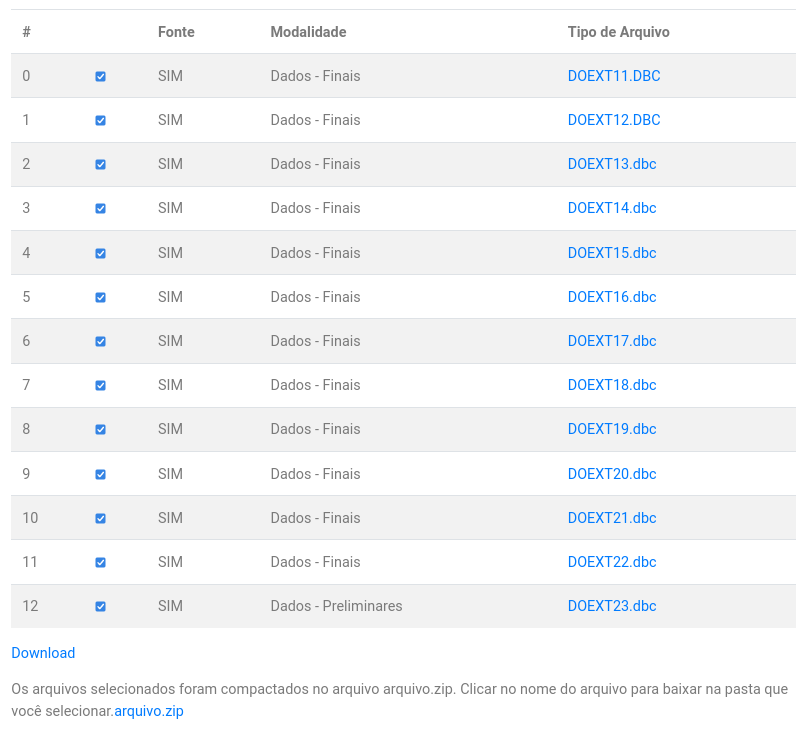
\includegraphics[width=11.17in]{../imgs/DATASUS} }

\subsection{}\label{section}

\subsection{Sinistros de trânsito na
CID-10}\label{sinistros-de-truxe2nsito-na-cid-10}

Causas de morte referentes a sinistros de trânsito são encontradas no da
\textbf{Classificação Estatística Internacional de Doenças e Problemas
Relacionados com a Saúde} (em inglês: \emph{International Statistical
Classification of Diseases and Related Health Problems -- ICD})
(\href{https://icd.who.int/browse10/2019/en\#/XX}{WHO, 2019}). Em sua
décima revisão, a chamada \textbf{CID-10} fornece códigos relativos à
classificação de doenças e de uma grande variedade de sinais, sintomas,
aspectos anormais, queixas, circunstâncias sociais e causas externas
para ferimentos ou doenças.

A imagem a seguir ilustra o \textbf{Capítulo XX -- Causas externas de
morbidade e de mortalidade} da CID-10 (à esquerda) e a categoria de
\textbf{Pedestres feridos em acidente de transporte (V01-V09)} (à
direita).

\href{https://icd.who.int/browse10/2019/en#/V01-V09}{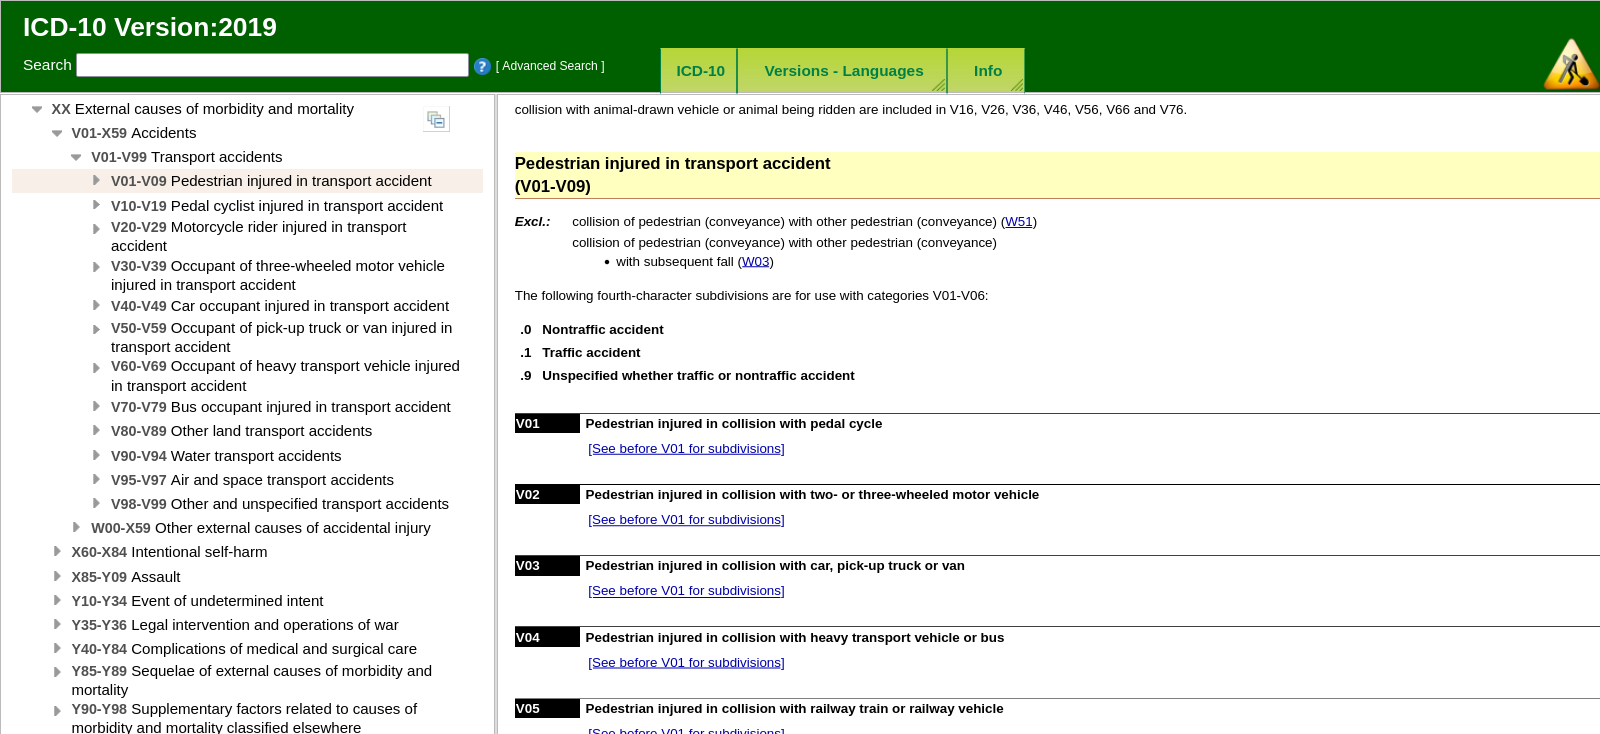
\includegraphics[width=22.22in]{../imgs/ICD-10} }

A imagem também mostra uma subdivisão dentro das causas básicas que é
relevante para o cômputo de mortes no trânsito. Ela é específica para
países cuja marcação da CID-10 possui uma quarta letra, como é o caso do
Brasil.

\begin{longtable}[]{@{}
  >{\centering\arraybackslash}p{(\columnwidth - 2\tabcolsep) * \real{0.3472}}
  >{\raggedright\arraybackslash}p{(\columnwidth - 2\tabcolsep) * \real{0.6528}}@{}}
\toprule\noalign{}
\begin{minipage}[b]{\linewidth}\centering
Quarta letra da CID-10
\end{minipage} & \begin{minipage}[b]{\linewidth}\raggedright
Subdivisão
\end{minipage} \\
\midrule\noalign{}
\endhead
\bottomrule\noalign{}
\endlastfoot
.0 & Acidente fora do trânsito {[}\emph{Nontraffic accident}{]} \\
.1 & Acidente em trânsito {[}\emph{Traffic accident}{]} \\
.9 & Não especificado se em trânsito ou fora dele {[}\emph{Unspecified
whether traffic or nontraffic accident}{]} \\
\end{longtable}

\begin{Shaded}
\begin{Highlighting}[]
\FunctionTok{summary}\NormalTok{(cars)}
\end{Highlighting}
\end{Shaded}

\begin{verbatim}
##      speed           dist       
##  Min.   : 4.0   Min.   :  2.00  
##  1st Qu.:12.0   1st Qu.: 26.00  
##  Median :15.0   Median : 36.00  
##  Mean   :15.4   Mean   : 42.98  
##  3rd Qu.:19.0   3rd Qu.: 56.00  
##  Max.   :25.0   Max.   :120.00
\end{verbatim}

\subsection{Including Plots}\label{including-plots}

You can also embed plots, for example:

\includegraphics{index_files/figure-latex/pressure-1.pdf}

Note that the \texttt{echo\ =\ FALSE} parameter was added to the code
chunk to prevent printing of the R code that generated the plot.

\subsection*{Referências}\label{referuxeancias}
\addcontentsline{toc}{subsection}{Referências}

\phantomsection\label{refs}
\begin{CSLReferences}{0}{1}
\bibitem[\citeproctext]{ref-who2020}
WHO, World Health Organization. \textbf{WHO methods and data sources for
country-level causes of death 2000-2019}. Geneva: World Health
Organization, 2020. Disponível em:
\href{https://www.who.int/docs/default-source/gho-documents/global-health-estimates/ghe2019_cod_methods.pdf}{https://www.who.int/docs/default-source/gho-documents/global-health-estimates/ghe2019\_cod\_methods.pdf.
}.

\bibitem[\citeproctext]{ref-who2022}
WHO, World Health Organization. \textbf{WHO Mortality Database}. Geneva,
2022. Disponível em:
\href{https://platform.who.int/mortality/themes/theme-details/topics/indicator-groups/indicator-group-details/MDB/road-traffic-accidents}{https://platform.who.int/mortality/themes/theme-details/topics/indicator-groups/indicator-group-details/MDB/road-traffic-accidents.
}

\end{CSLReferences}

\end{document}
